\chapter{Metodología (\tb{Problem Formulation})}

El objetivo del trabajo es estabilizar un UAV usando algoritmos de control basados en una red neuronal entrenada empleando algoritmos de aprendizaje automático. Los principales componentes que intervienen en el agente son el estado, las acciones y la recompensa, para cada problema hay un conjunto que estados, acciones y funciones de recompensa que pueden llevar a que el agente aprenda.

\section{Diseño del estado}
 El autopiloto cuenta con 2 IMUs para poder obtener datos sobre su estado. Se quiere estabilizar el dron en una orientación concreta, por lo tanto el estado que se ha diseñado consta de 6 parámetros:
\begin{equation}
	S=(\varphi,\theta,\psi,\dot\varphi,\dot\theta,\dot\psi) \qquad\qquad \varphi,\theta,\psi,\dot\varphi,\dot\theta,\dot\psi \in [-1,1]
\end{equation} 

Siendo $\varphi,\theta$ y $\psi$ los ángulos de alabeo (\textit{roll}), cabezeo (\textit{pitch}) y guiñada (\textit{yaw}) del dron  y $\dot\varphi,\dot\theta$ y $\dot\psi$ sus respectivas velocidades. Para favorecer la convergencia del aprendizaje, se ha normalizado el estado para que todas sus componentes estén comprendidas dentro del intervalo $[-1,1]$.

Los ángulos proporcionan información sobre el estado actual y la velocidad angular sobre los estados pasados y los posibles estados futuros, es decir, proporciona cierta información temporal. 

\section{Diseño de las acciones}
Al trabajar con un quadricóptero podemos actuar sobre la potencia que se le entrega a los motores, por lo que cada acción que realice el agente constará de 4 campos:
\begin{equation}
	A = (T_1,T_2,T_3,T_4) \qquad\qquad T_i \in [-1,1]
\end{equation}

Siendo $T_i$ la potencia \textit{(Thrust)} normalizada entregada a cada motor. Un valor de $T_1=-1$ significa que el motor 1 estaría girando a la mínima potencia permitida y un valor de $T_1=1$ corresponde a que el motor 1 estaría girando a la máxima potencia.\\

Las señales de control que admiten los variadores es una señal PWM de 50Hz cuyo ancho de pulso debe estar entre 1ms y 2ms. Un ancho de pulso de 1ms se corresponde con la mínima velocidad el motor y un ancho de 2ms con la máxima, veáse \cref{hardware_ESCWAVE}.\newpage

\begin{figure}[htb!]
	\centering
	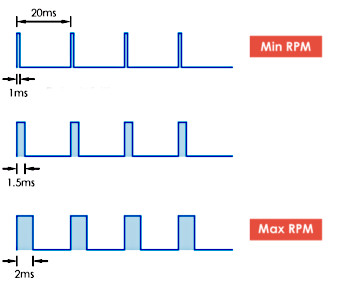
\includegraphics[width=0.6\textwidth]{hardware/ESCWaves}
	\caption{Formas de onda que recibe un variador}
	\label{hardware_ESCWAVE}	
\end{figure}

 Para realizar esta transformación del dominio $[-1,1]$ al dominio [1000,2000] $\mu$s se han empleado la siguiente expresión

\begin{equation}
	P_i= T_i \cdot 1000 \cdot \alpha + \beta \qquad \qquad i=0,...,3
\end{equation}\\
siendo $P_i$ el ancho del pulso enviado al ESC, $\alpha \in [0,1]$  es el porcentaje de la potencia total que puede manejar el controlador y $\beta \in [0,2000]$ es la velocidad base que tienen los motores. Esta velocidad base permite que el dron pueda variar su altura y que se pueda autosustentar. 

\section{Diseño de la función de recompensa}
La función de recompensa rige la forma en la que la red va a configurar sus pesos, por lo tanto, cómo se va a comportar el agente en un estado determinado.
Para conseguir que el agente responda de la forma deseada se han probado una gran variedad de funciones de \textit{reward}, optando finalmente por:
\begin{equation}
	%R_t = \left( 1-\frac{|\varphi - \varphi_{ref}| + |\theta-\theta_{ref}| + |\psi- \psi_{ref}|}{3}\right)^3
	R_t = \left( 1-\frac{|\varphi|  + |\theta| + |\psi|}{3}\right)^3
\end{equation}
Con esta funcion de recompensa \tb{BLA BLA BLA}

